\textbf{Parallel Design}: Figure~\ref{figs:parallelmd} illustrates the design of NAMD decomposition.
The parallel structure of NAMD is based on a unique object-based
hybrid decomposition, parallelized using the \charmpp{} programming model.
Atomic data is decomposed into spatial domains (called ``patches''
shown in yellow box in figure) based on the short-range
interaction cutoff distance such that in each dimension only atoms in
one-away or, when necessary to increase concurrency, one-away and two-away
neighboring domains will interact directly.
These equally-sized domains are distributed as evenly as possible across
the machine and are responsible for accumulating forces and integrating
the equations of motion asynchronously via per-domain user-level threads.
Patches are represented on other cores by proxies and all position
and force data sent between cores passes via these proxy patches.

The calculation of short-range interactions is orthogonally decomposed
into ``compute objects'' (shown in red diamond) representing interactions between atoms within
a single domain, between pairs of domains, or for groups of neighboring
domains for terms representing multi-body covalent bonds.
Compute objects are scheduled by local prioritized \charmpp{} messages
when updated position data is received for all required patches.
Longer-running domains are further subdivided by partitioning their outer
interaction loops to achieve a grain-size that enables both load balancing
and interleaving of high-priority PME or remote-atom work with
lower-priority work that does not require off-node communication.

\begin{figure}[h]
\centering
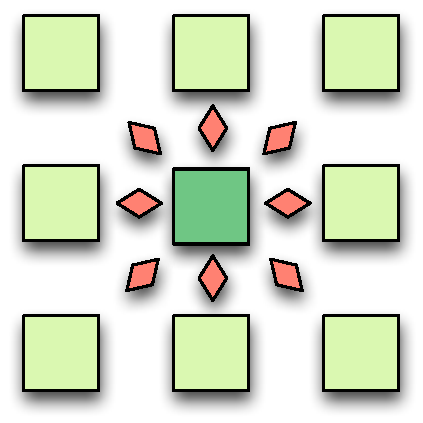
\includegraphics[width=2.8in]{figs/parallelmd}
\caption{NAMD decomposition}
\label{figs:parallelmd}
\vspace{-0.2cm}
\end{figure}

\textbf{GPU and CPU work assignment}:
NAMD offloads only short-range non-bonded calculations to the GPU
as these are the most expensive part of the calculation, are best suited
to the GPU architecture, and do not require additional communication stages.
Every non-bonded compute object assigned to a given GPU is mapped to one or
two GPU multiprocessor work units (``blocks'' in CUDA).
Although GPUs support very fine-grained parallel decomposition internally,
the interface presented to the controlling CPU requires data and work to
be aggregated for efficiency.
When all required position data is received on the CPU, it is then copied
to the GPU and two sets of work units are scheduled.
The first set calculates forces for remote atoms, which require off-node
communication, and the second set calculates only forces for local atoms.
This allows some overlap of communication and computation~\cite{phillips_stone_namd_cuda}.



